\documentclass[11pt]{article} 
\usepackage{bm}
\usepackage{cmap}
\usepackage{ctex}
\usepackage{cite}
\usepackage{color}
\usepackage{float}
\usepackage{xeCJK}
\usepackage{amsthm}
\usepackage{amsmath}
\usepackage{amssymb}
\usepackage{setspace}
\usepackage{geometry}
\usepackage{hyperref}
\usepackage{enumerate}
\usepackage{indentfirst}
\usepackage{yfonts}
\usepackage{pdfpages}
\usepackage{ulem}
\usepackage{hyperref}

\usepackage[cache=false]{minted}

% 代码高亮
\geometry{margin=1in}

\newcommand{\verilogcode}[1]
{
  \inputminted[mathescape,
  tabsize=4,
  linenos,
  % frame=single,
  framesep=2mm,
  breakaftergroup=true,
  breakautoindent=true,
  breakbytoken=true,
  breaklines=true,
  fontsize=\small
  ]{verilog}{#1}
}

\title{计算机体系结构(1)大作业报告\thanks{https://github.com/lmxyy/Computer-Architecture-Task-2}}
\author{李沐阳 \quad 516021910346\\ \emph{Shanghai Jiao Tong University}
}
\date{\today}

\begin{document}

\maketitle
\newpage

\section{设计思路}
\label{sec:设计思路}

设计整体思路是按照《自己动手写CPU》的实现的一个Riscv五级流水。相对于普通的mips五级流水,本cpu去掉了一些历史包袱,如延迟槽,HI/LO寄存器等等。本cpu使用的是冯诺依曼结构(即指令也存放与内存中)。具体实现思路如下:
\begin{figure}[h]
  \centering
  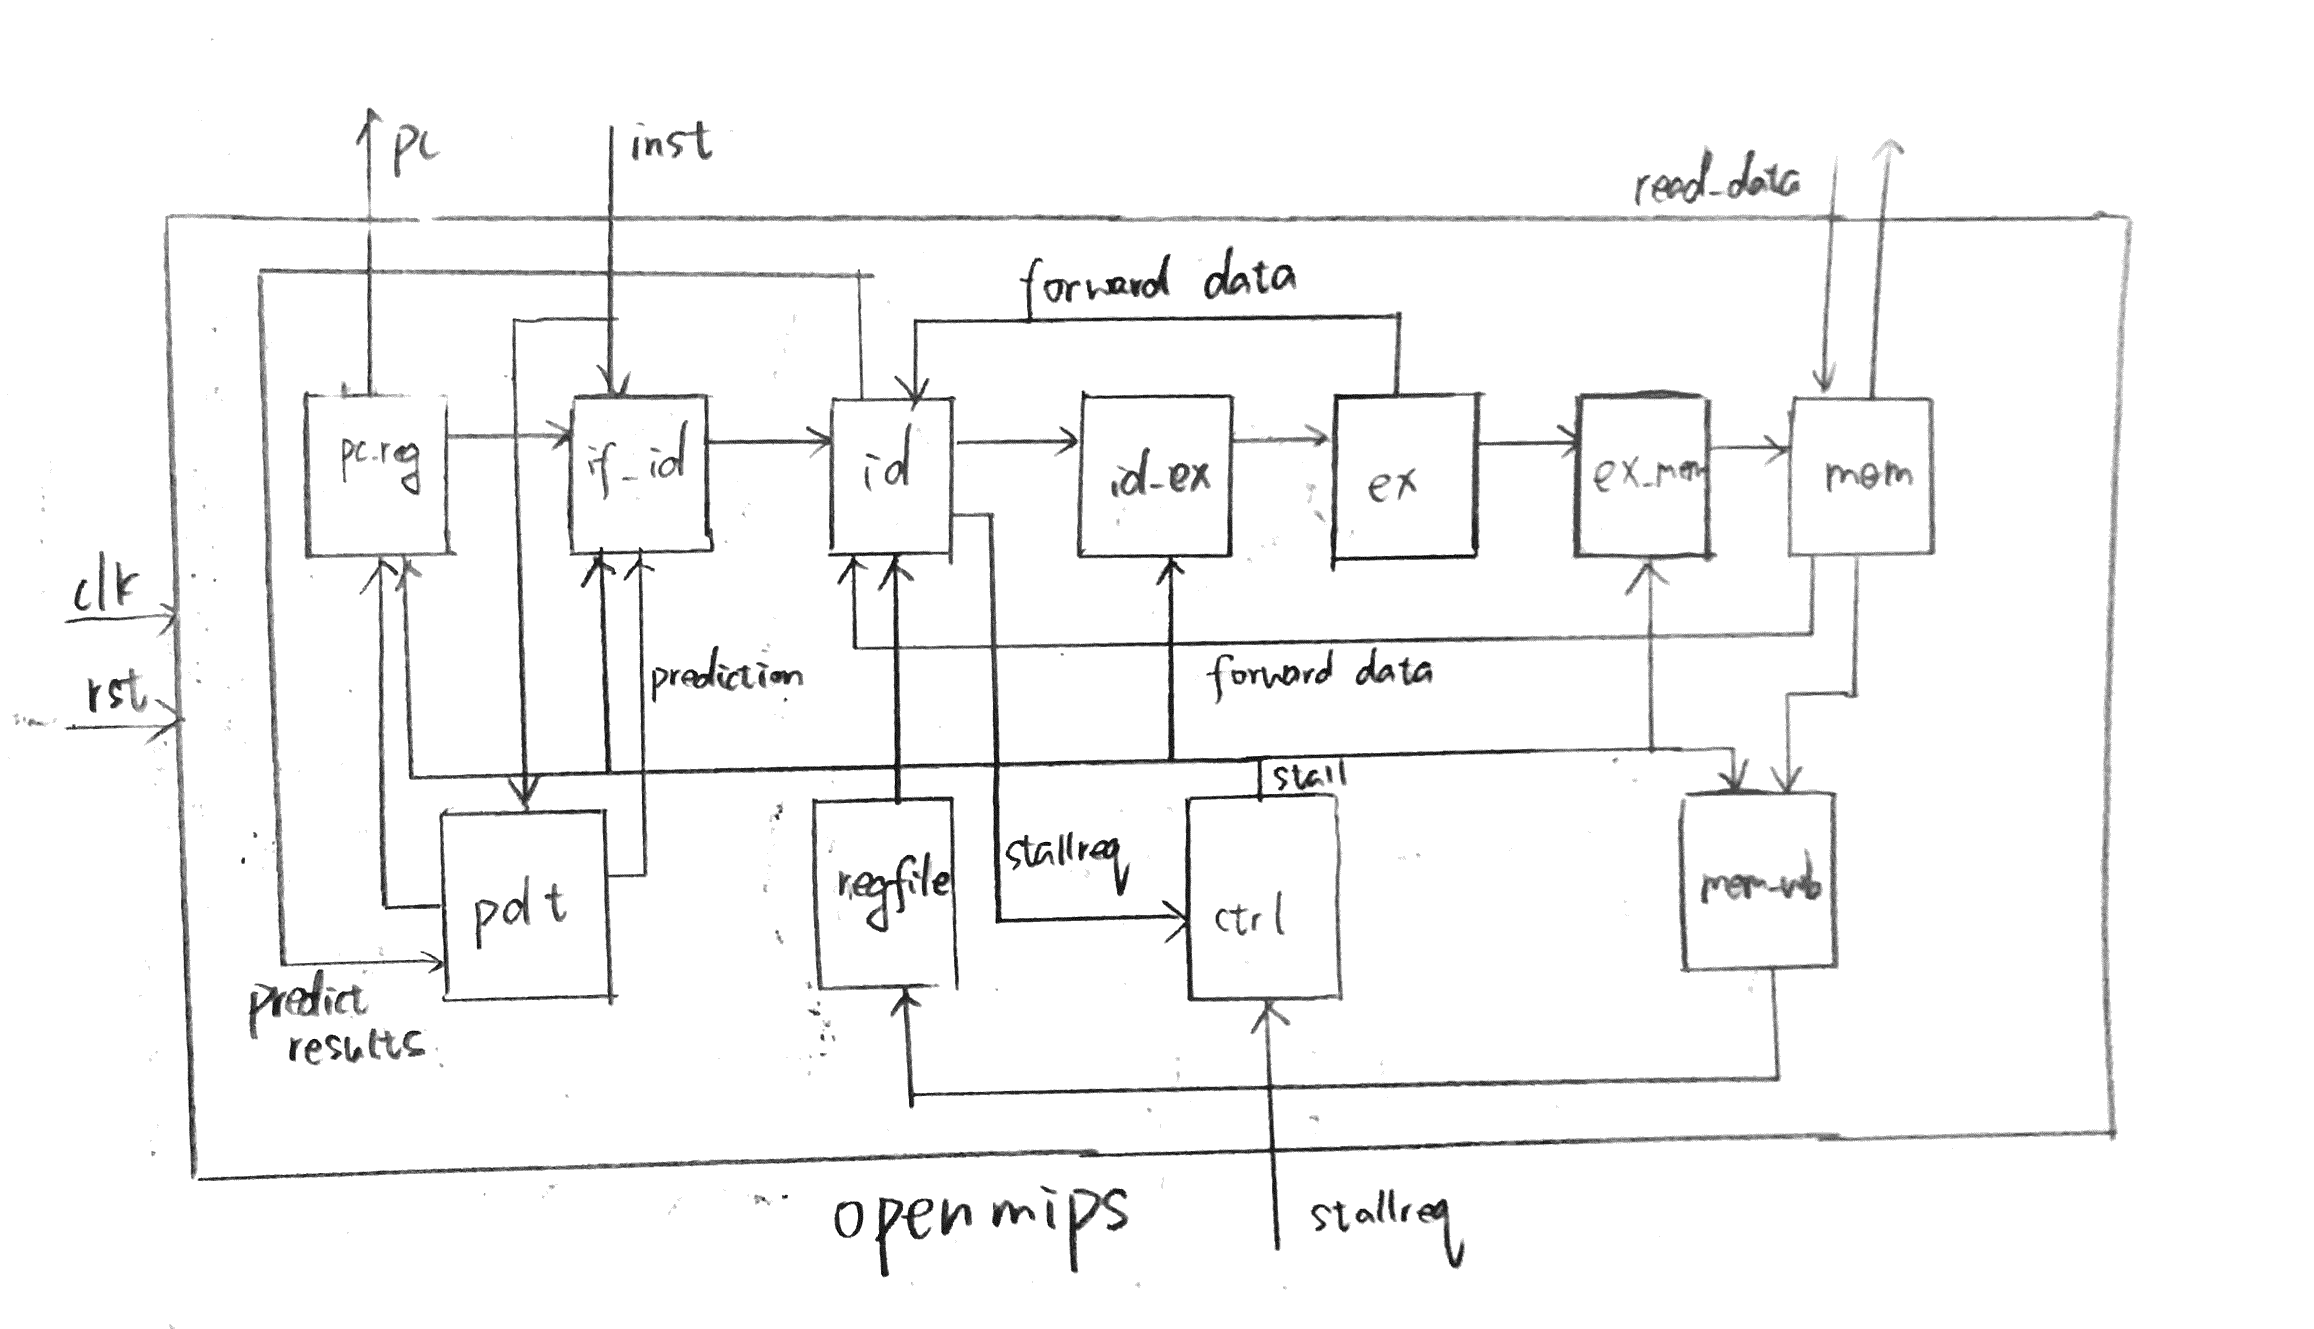
\includegraphics[scale=0.12]{../Picture/openmips.png}
  \caption{openmisp示意图}
  \label{fig:openmips}
\end{figure}

\begin{figure}[h]
  \centering
  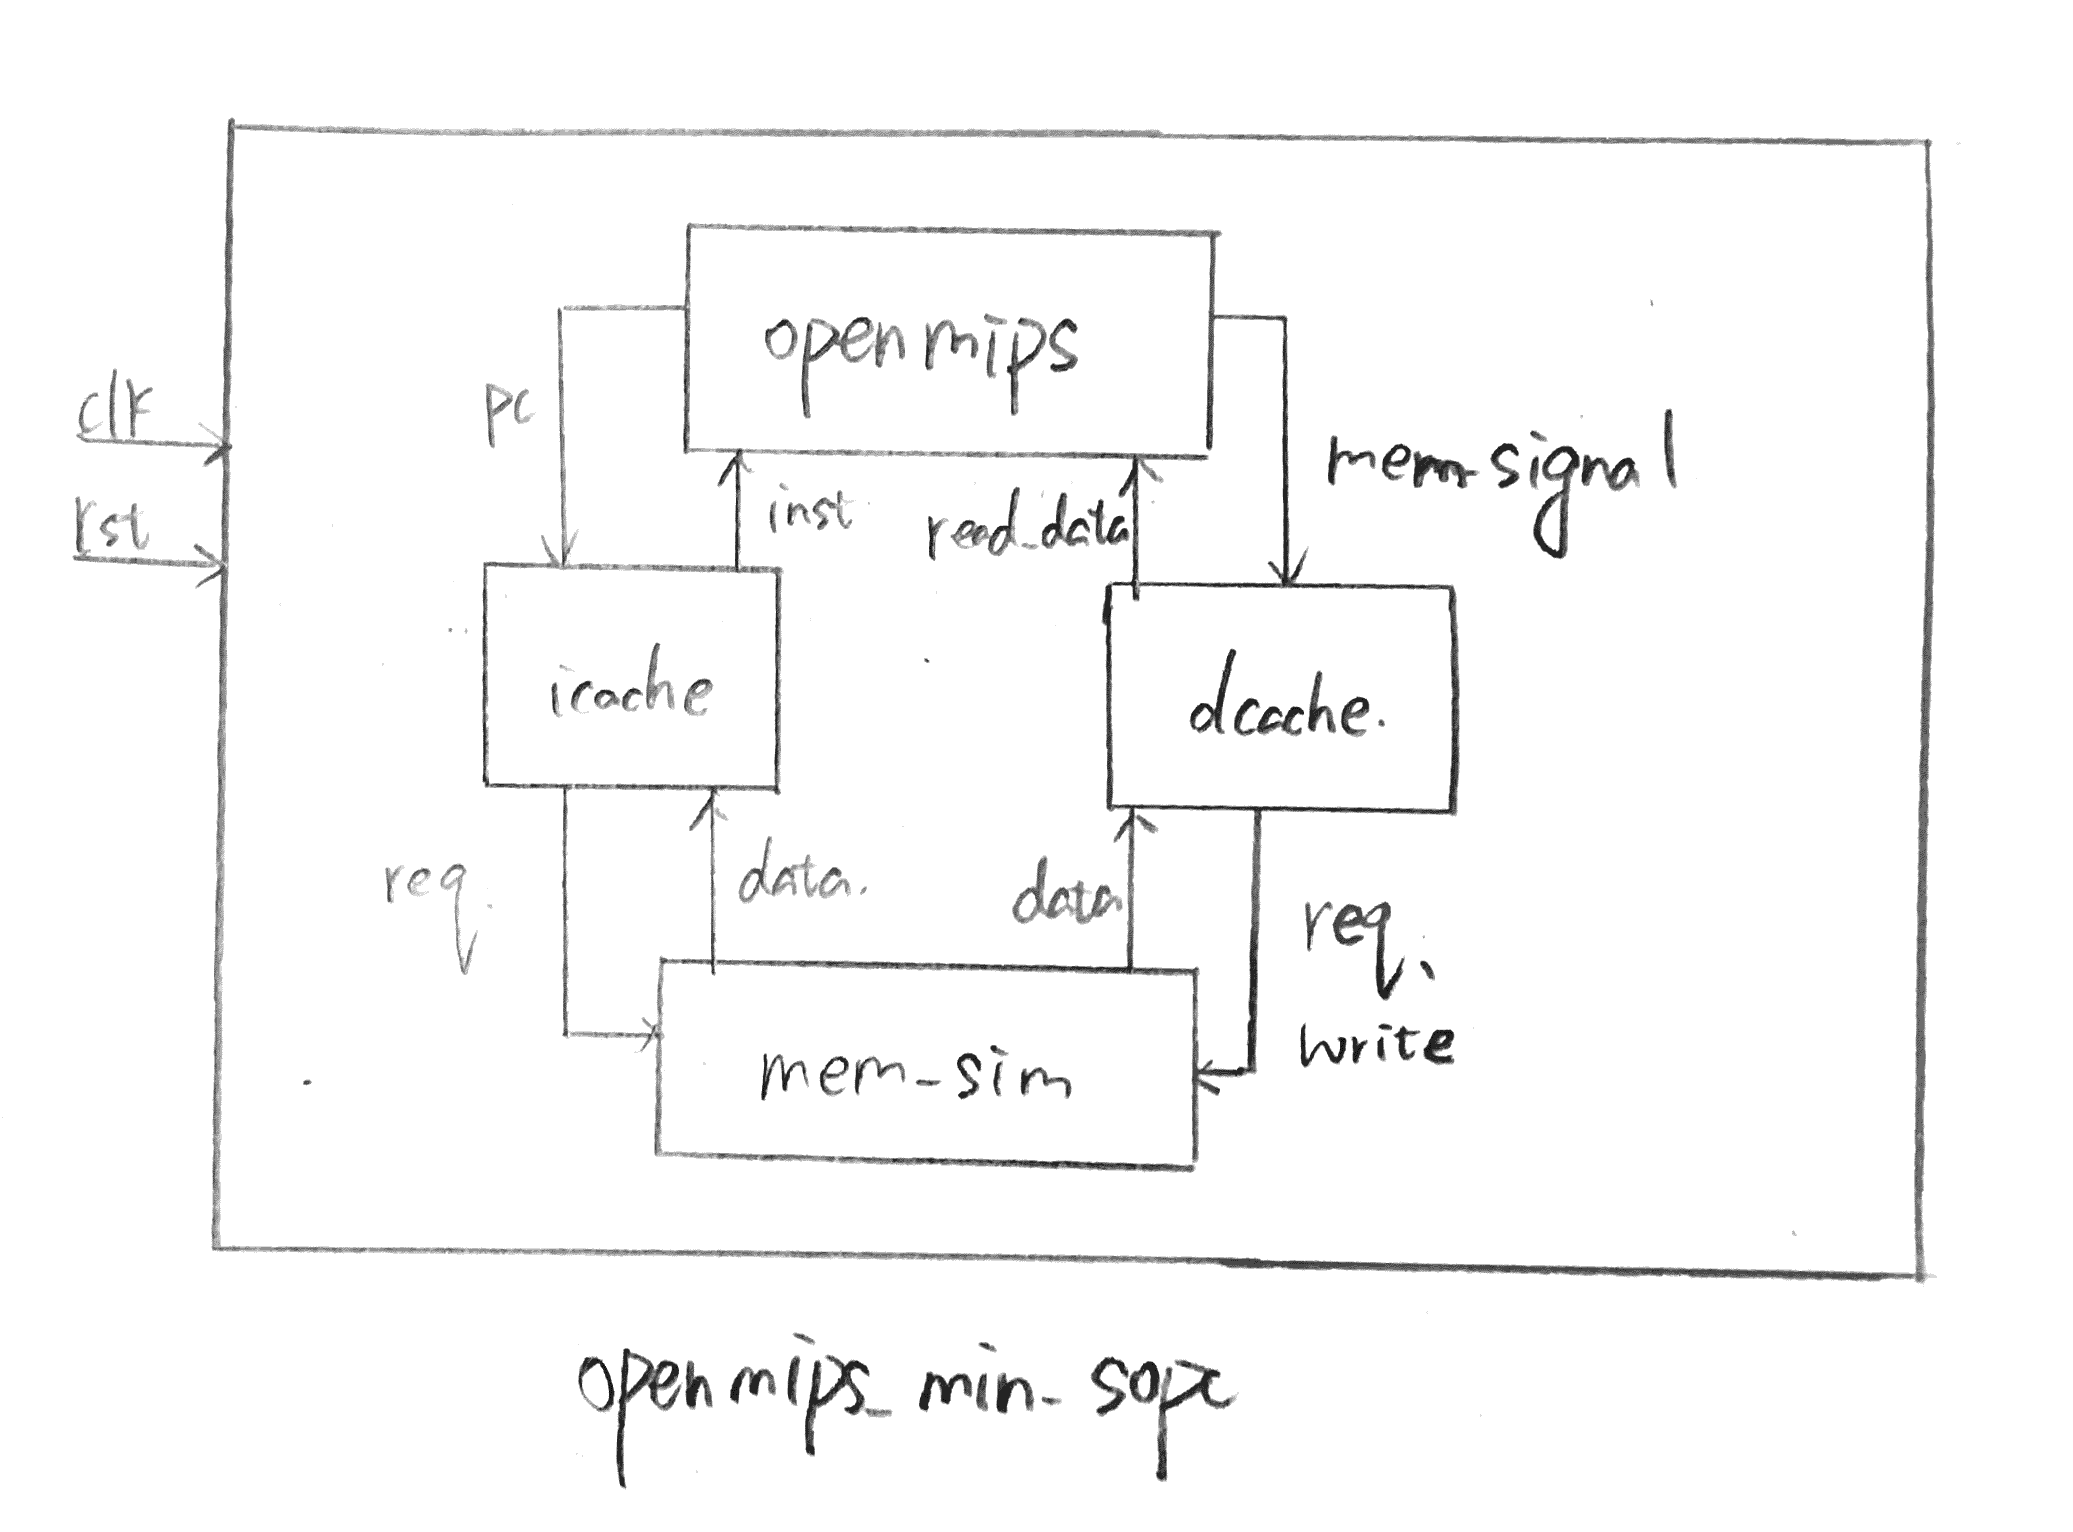
\includegraphics[scale=0.12]{../Picture/openmips_min_sopc.png}  
  \caption{openmips\_min\_sopc示意图}
  \label{fig:openmips_min_sopc}
\end{figure}
\newpage{}
\section{创新之处}
\label{sec:创新之处}

\subsection{分支预测器}
\label{sec:分支预测器}

pdt模块为一个分支预测器——它采用的是Tournament的预测策略:
\begin{itemize}
\item 根据pc地址的2$\sim$11位,选择一个alloyed branch predictor的两位饱和计数器,由此判断使用全局预测器还是局部预测器;
\item 若使用全局计数器,则直接根据最近10次分支结果,选择相应的全局饱和计数器。
\item 若使用局部计数器,则根据pc地址后2$\sim$11位\textbf{以及最近三次分支结果},选择相应的饱和计数器。\sout{(我猜这样准确率更高)}
\end{itemize}
Predict过程在if阶段就得完成,同时将结果传到pc和id阶段。id阶段分支结果出来后,也应相应地对预测器产生相应的反馈。

\subsection{Cache}
\label{sec:Cache}
\begin{itemize}
\item 两路主关联cache,每块中放8Bytes,index位长度可调;
\item 替换策略:LRU;
\item Write策略:Write through,同时只有读不命中时才会产生替换。
\item 若需要替换,cache会使cpu暂停直到替换结束且数据读出(icache将if暂停,dcache将除了wb以外的阶段全部暂停);
\item 由于实现的是内存模拟器,故可以连多根线到内存。所以icache和dcache可以同时从内存中读取数据,不需要stall。
\end{itemize}
\section{遇到问题}
\label{sec:遇到问题}

\subsection{Cache问题}
\label{sec:Cache问题}

我的Cache虽然很简单,但是实现起来费了很大的劲,尤其是时序一直弄不对,always的条件一直不知道该怎么填写。我现在虽然Cache能够正确跑出结果,但是还是不能明白其中的原理,感觉是瞎改改出来的:

我的icache.v里有这样一段代码:
\verilogcode{example.v}
若改为上升沿clk触发,那么我每次pc=0该stall的时候,pc值都会莫名其妙变为了4。我感觉应该是在stall信号来之前,pc先加了4。改成了clk触发,就没了这样的情况。

\subsection{通讯问题}
\label{sec:通讯问题}
在我的adapter里,我如果写内存,我就需要发送至少9Bytes的数据。而助教的uart buffer只有8Bytes。故无法做到将数据存入缓冲,流水继续执行,必须得stall到第9个数据也存入buffer之中。我的想法是需要把这个缓冲扩大,但我不知道助教为什么缓冲开到8就足够了。

\subsection{一些想法}
\label{sec:一些想法}

在五级流水之中,如果实现了像tomasulo那样的寄存器表用于rename,在data forward的时候打上相应tag,我感觉或许可以很大程度上面减少stall的节拍。

\section{特别感谢}
\label{sec:特别感谢}
\begin{itemize}
\item 张凯羿同学提供的技术上的支持。
\item 范舟同学提供的数据上的支持。
\end{itemize}
\begin{thebibliography}{9}
\bibitem{} \protect{\href{https://github.com/lmxyy/Computer-Architecture-Task-2/blob/master/Document/%E3%80%8A%E8%87%AA%E5%B7%B1%E5%8A%A8%E6%89%8B%E5%86%99CPU%E3%80%8BP1-300.pdf}{《自己动手写CPU》}}
\bibitem{} \protect{\href{https://github.com/lmxyy/Computer-Architecture-Task-2/blob/master/Document/riscv-spec-v2.2.pdf}{riscv-spec-v2.2.pdf}}
\bibitem{} \protect{\href{https://en.wikipedia.org/wiki/Branch_predictor#Glob...}{Branch Prediction Wikipedia}}
\bibitem{} \protect{\href{https://github.com/sxtyzhangzk/mips-cpu/}{助教的MIPS CPU实现}}
\bibitem{} \protect{\href{https://github.com/sxtyzhangzk/cpu-judge}{cpu-judge}}
\bibitem{} \protect{\href{https://github.com/lmxyy/Computer-Architecture-Task-2/blob/master/Document/Basys3-FPGA-%E5%BC%80%E5%8F%91%E6%9D%BF%E5%AE%9E%E9%AA%8C%E5%8F%82%E8%80%83%E8%B5%84%E6%96%99.pdf}{Basys3-FPGA-开发板实验参考资料}}
\end{thebibliography}
\end{document}
